\documentclass[11pt]{article}
\usepackage[hyperref]{acl} % Ensure you have the acl.sty file in your directory
\usepackage{times}
\usepackage{latexsym}
\usepackage{microtype}
\usepackage{booktabs}
\usepackage{enumitem}
\usepackage{amsmath}
\usepackage{float}    % Required for [H]
\usepackage{graphicx} % Added for including figures
% Required packages (add these to your preamble if not already present):
\usepackage{amsmath}
\usepackage{tikz}
\usepackage{float}
% \usepackage{natbib} % Required for acl_natbib.bst

\usetikzlibrary{shapes.geometric, arrows, positioning, shadows}
% Define block styles
\tikzstyle{process} = [rectangle, minimum width=4cm, minimum height=1cm, text centered, text width=4.5cm, draw=black, fill=blue!5, rounded corners, drop shadow]
\tikzstyle{arrow} = [thick,->,>=stealth]

\bibliographystyle{acl_natbib}

\title{Transportation Mobility Insights: Predictive Modeling of Taxi Tip Amounts}

\author{
  \textbf{Zhiqiang Ni, Tony Xue, Xiao Du} \\
  \vspace{0.25em}
  Michigan State University \\
  \texttt{\{nizhiqia, xuetony, duxiao\}@msu.edu} % Placeholder emails - recommended for ACL style
}

\begin{document}
\begin{titlepage}
    \centering
    \vspace*{2cm}

    % Project Title
    {\Huge \textbf{Transportation Mobility Insights: \\ Predictive Modeling of Taxi Tip Amounts} \par}

    \vspace{2.5cm}

    % Difficulty Level
    {\LARGE \textbf{Difficulty Level:} Moderate \par}

    \vspace{2.5cm}

    % Team Contributions
    {\Large \textbf{Team Member Contributions} \par}
    \vspace{1cm}

    \begin{itemize}[label={}, leftmargin=0.25\textwidth]
        \item \textbf{Zhiqiang Ni:} \dotfill [e.g., Data Cleaning, Model A]
        \vspace{0.5cm}
        \item \textbf{Tony Xue:} \dotfill [e.g., Visualization, Analysis]
        \vspace{0.5cm}
        \item \textbf{Xiao Du:} \dotfill [e.g., Report Writing, Model B]
    \end{itemize}

    \vfill

    % Institution & Date
    {\large Michigan State University \par}
    \vspace{0.5cm}
    {\large \today \par}

    \vspace*{1cm}
\end{titlepage}
\maketitle

\begin{abstract}
This project explores how ride characteristics and environmental factors influence tipping behavior in New York City taxis. Using publicly available NYC Taxi and Limousine Commission (TLC) datasets covering \textbf{green and yellow taxis from 2024}, combined with historical weather data, we aim to predict whether a ride receives a \textit{low}, \textit{medium}, or \textit{high} tip. We begin with Initial Data Analysis (IDA) to understand data quality and structure, identify missing or inconsistent entries, and engineer key features such as trip duration, distance, tip ratio, and weather conditions.

After cleaning and transformation, we trained multiple classification models, including Logistic Regression, Random Forests, Histogram Gradient Boosting, and a custom neural network implemented in PyTorch. The goal is to build a predictive system that reveals how ride and environmental factors jointly affect tip behavior.

Finally, we deployed a \textbf{Weighted Ensemble} mechanism within an interactive application to synthesize predictions from all models. The goal of this project is not only to build a reliable classification model but also to uncover the key ride and environmental factors that drive tipping behavior, providing interpretable insights into passenger generosity.
\end{abstract}

\section{Introduction}

Understanding the factors that drive consumer tipping behavior is a question of both economic and social significance. In urban transportation systems, tips constitute a substantial portion of driver income, yet the mechanisms governing when and how much passengers tip remain incompletely understood. New York City generates millions of rides annually, each representing a micro-transaction that reflects passenger generosity, service quality, and situational context.

This project investigates the predictive power of ride characteristics and environmental factors in determining tip amounts for NYC taxi rides. While prior work has examined tipping in service industries broadly, the availability of large-scale, granular taxi trip data—combined with historical weather information—presents a unique opportunity to quantify the interplay between trip attributes and external conditions.

\subsection{Motivation}

The motivation for this research is threefold. First, from a \textit{driver perspective}, understanding tip determinants can inform strategic decisions about when and where to operate. Second, from an \textit{analytical perspective}, taxi trip data provides a rich testbed for classification algorithms, with inherent challenges including class imbalance and feature engineering. Finally, we aim to operationalize these insights by deploying a user-friendly interface for real-time prediction.
\subsection{Challenges}

This project confronts several key analytical challenges:

\begin{enumerate}
    \item \textbf{Data Volume and Quality}: Processing over 3 million trip records from multiple data sources (Yellow Taxi, Green Taxi, and weather API) requires efficient data handling and careful validation to remove anomalies, outliers, and invalid entries.

    \item \textbf{Missing Data}: Real-world datasets inherently contain missing values. Applying appropriate imputation strategies while preserving underlying data distributions is critical for model integrity.

    \item \textbf{Feature Engineering}: Raw taxi data must be transformed into meaningful predictive features. This includes deriving temporal attributes (hour, day of week), trip metrics (speed, duration), and integrating external weather variables with appropriate time-based joins.

    \item \textbf{Class Imbalance}: Tip distributions are often skewed, with certain tip ranges (e.g., standard 15-20\%) being far more common than extreme low or high tips. This imbalance can bias model predictions toward majority classes.

    \item \textbf{Model Selection and Comparison}: Evaluating multiple classification algorithms—from traditional methods like Logistic Regression to ensemble approaches like Random Forests and gradient boosting—requires systematic comparison on consistent metrics.
\end{enumerate}

\subsection{Project Goal}

The primary goal of this project is to develop and evaluate a suite of machine learning models capable of predicting tip classifications (low, medium, high) based on trip and environmental features. Specifically, we aim to:

\begin{itemize}
    \item Construct a clean, integrated dataset combining 2024 NYC taxi records with hourly weather data
    \item Engineer interpretable features that capture temporal, spatial, trip-specific, and weather-related patterns
    \item Train and rigorously compare eight distinct classification models (including traditional ML and deep learning approaches)
    \item Identify which features most strongly influence tipping behavior
    \item Deploy an interactive dashboard for exploratory analysis and real-time prediction
\end{itemize}

Beyond prediction accuracy, we seek \textit{interpretability}—understanding not just \textit{what} the models predict, but \textit{why}. Feature importance analysis and visualization of decision boundaries will illuminate the relative contributions of different factors, providing actionable insights for drivers and policymakers alike.

\subsection{Contributions and Findings}
This project makes several key contributions to the understanding of taxi tipping behavior and predictive modeling of service tips. We developed an end-to-end pipeline for collecting, cleaning, and preprocessing multi-source transportation data. By analyzing over 3 million sampled taxi trips with robust feature engineering, we provide an extensive empirical study of tipping behavior.

From a modeling perspective, we systematically evaluated eight machine learning algorithms. Our results demonstrate that the \textbf{Histogram Gradient Boosting model achieves the highest accuracy at 66.68\%}. This ensemble approach effectively captures the non-linear relationships in the data and outperforms traditional linear models, demonstrating strong balanced performance across all tip classes, particularly for high-value tips.

To enhance the practical utility of this research, we deployed a public Streamlit web application. This interactive tool allows users to visualize correlations, explore temporal patterns, and input custom trip parameters to receive real-time tip class predictions, bridging the gap between theoretical modeling and end-user application.


\section{Related Work}
This project builds upon distinct streams of literature: the economic and social motivations behind tipping, the specific influence of environmental factors on transportation behaviors, and advanced statistical methods for handling incomplete multivariate data.

\subsection{Theoretical Foundations of Tipping}
Tipping represents a unique economic transaction that differs significantly from standard pricing mechanisms. While tips are theoretically discretionary, they function largely as a social norm rather than a purely rational economic calculation \citep{azar2020economics}. \citet{azar2020economics} argues that the ``future-service'' hypothesis---the idea that customers tip to ensure good service on their next visit---is unsupported by empirical evidence, as tipping behaviors do not significantly differ between repeat and one-time customers. Instead, tipping is driven by psychological motivations, such as the desire to avoid embarrassment, the need to adhere to established social norms, and the desire to show gratitude \citep{azar2020economics}. In the United States specifically, the tipping norm has evolved significantly, with standard rates rising from 10\% in the early 20th century to 15--20\% in recent decades \citep{azar2020economics}.

\subsection{Weather Impacts on Mobility and Tipping}
The relationship between weather and consumer behavior in the transportation sector is complex. Research on ride-hailing services indicates that weather conditions significantly alter ridership patterns. For example, \citet{LIU2021257} found that precipitation positively impacts ride-hailing ridership, while increased wind speed exerts a negative influence. Furthermore, the flexibility of ride-hailing supply allows it to adjust to these weather changes more dynamically than traditional public transit \citep{LIU2021257}.

Regarding the specific impact of weather on \textit{tipping}, the literature presents conflicting findings. Early psychological research suggested that pleasant weather (sunshine) improves mood and subsequently increases tipping \citep{flynn2012weather}. However, \citet{flynn2012weather} challenged this ``mood-mediation'' theory, finding no statistically significant relationship between sunshine and tipping rates in restaurant settings when using actual weather data. They argued that tipping is better explained as an institutional standard rather than a behavior modulated by weather-induced mood changes \citep{flynn2012weather}.

Conversely, recent studies utilizing large-scale taxi data suggest a ``reciprocity'' effect. \citet{LEE2020101458}, analyzing NYC taxi data, found that passengers tend to be more generous tippers during extreme weather events, such as heavy precipitation or extreme temperatures. They propose that this generosity stems from ``driver-induced reciprocity,'' where passengers recognize the extra effort and risk drivers undertake during inclement conditions and tip more to restore equity \citep{LEE2020101458}.

\subsection{Methodological Approaches to Missing Data}
Real-world transportation datasets frequently contain missing values, necessitating robust imputation strategies to preserve statistical power. The method of Multiple Imputation by Chained Equations (MICE), or Fully Conditional Specification (FCS), has emerged as a preferred technique for complex multivariate data \citep{JSSv045i03}. Unlike joint modeling, which assumes a specific multivariate distribution for the entire dataset, MICE specifies imputation models on a variable-by-variable basis. This approach allows for the preservation of relations within the data and appropriately models the uncertainty inherent in the missing values \citep{JSSv045i03}. Research indicates that FCS is particularly attractive when no suitable multivariate distribution can be found for the data, making it highly effective for heterogeneous datasets involving both categorical and numerical variables \citep{JSSv045i03}.

\section{Methodology}
The primary objective is a multi-class classification task: predicting the ``generosity'' of a passenger's tip based on trip characteristics and environmental factors. By accurately classifying trips into \textbf{Low}, \textbf{Middle}, or \textbf{High} tip categories, this analysis aims to provide actionable insights for drivers to optimize earnings and for policymakers to understand economic behaviors in transportation. The overall data science workflow implemented in this project, from data ingestion to model evaluation, is summarized in Figure \ref{fig:methodology_pipeline}.

\begin{figure}[H]
\centering
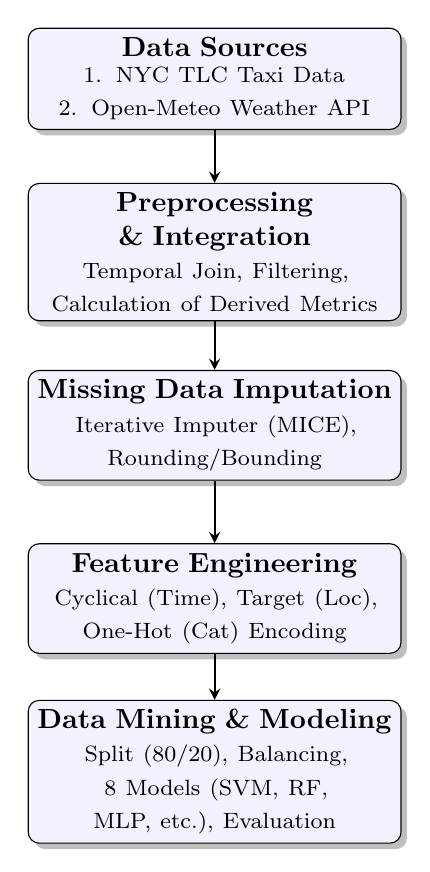
\begin{tikzpicture}[node distance=2.2cm]

% Nodes
\node (sources) [process] {\textbf{Data Sources}\\ \footnotesize 1. NYC TLC Taxi Data\\ 2. Open-Meteo Weather API};

\node (integration) [process, below of=sources] {\textbf{Preprocessing \& Integration}\\ \footnotesize Temporal Join, Filtering, Calculation of Derived Metrics};

\node (impute) [process, below of=integration] {\textbf{Missing Data Imputation}\\ \footnotesize Iterative Imputer (MICE), Rounding/Bounding};

\node (feature) [process, below of=impute] {\textbf{Feature Engineering}\\ \footnotesize Cyclical (Time), Target (Loc), One-Hot (Cat) Encoding};

\node (model) [process, below of=feature] {\textbf{Data Mining \& Modeling}\\ \footnotesize Split (80/20), Balancing, 8 Models (SVM, RF, MLP, etc.), Evaluation};

% Arrows
\draw [arrow] (sources) -- (integration);
\draw [arrow] (integration) -- (impute);
\draw [arrow] (impute) -- (feature);
\draw [arrow] (feature) -- (model);

\end{tikzpicture}
\caption{Schematic diagram of the data processing and modeling pipeline.}
\label{fig:methodology_pipeline}
\end{figure}

\subsection{Data Collection and Description}
The dataset was constructed by integrating three distinct sources to capture both transactional details and environmental context:

\begin{enumerate}
    \item \textbf{Yellow Taxi Trip Records (2024):} Sourced from the NYC Taxi \& Limousine Commission (TLC), representing traditional street-hail taxis primarily in Manhattan.
    \item \textbf{Green Taxi Trip Records (2024):} Sourced from the TLC, representing ``Boro Taxis'' that serve outer boroughs and northern Manhattan.
    \item \textbf{Historical Weather Data:} Hourly weather metrics (temperature, precipitation, wind speed, snowfall, weather code) retrieved via the Open-Meteo API for New York City coordinates ($40.7834^\circ$N, $-73.9663^\circ$W).
\end{enumerate}

The raw taxi datasets contain granular features including pickup/dropoff timestamps, geolocation IDs (\texttt{PULocationID}, \texttt{DOLocationID}), passenger counts, trip distances, and detailed fare breakdowns (fare amount, extra, tax, tip amount).

\subsection{Data Preprocessing}
Extensive preprocessing was required to ensure data quality and relevance. The cleaning process involved the following steps:

\begin{itemize}
    \item \textbf{Data Cleaning:} Records containing negative total amounts, zero trip distances, or negative time durations were removed. Trips paid via cash (\texttt{payment\_type} = 2) were excluded, as tip amounts are not reliably recorded for these transactions. Furthermore, unrealistic trips with calculated average speeds exceeding 100 mph were filtered out as outliers or measurement errors.

    \item \textbf{Target Variable Creation:} The target variable, \texttt{tip\_class}, was derived from the tip percentage, calculated as:
    \begin{equation}
        \text{tip\_pct} = \frac{\text{tip\_amount}}{\text{total\_amount} - \text{tip\_amount}}
    \end{equation}
    The continuous percentage was discretized into three classes:
\begin{itemize}
        \item \textbf{Low (0):} $\text{tip\_pct} \leq 0.10$ (0--10\%)
        \item \textbf{Middle (1):} $0.10 < \text{tip\_pct} \leq 0.20$ (10--20\%)
        \item \textbf{High (2):} $\text{tip\_pct} > 0.20$ (Over 20\%)
    \end{itemize}

    \item \textbf{Data Integration:} The taxi and weather datasets were merged using a left join on the pickup timestamp, rounded to the nearest hour, ensuring every trip was associated with the concurrent weather conditions.
\end{itemize}

\subsection{Missing Data Imputation}
To address missing values in critical features (e.g., \texttt{passenger\_count}, \texttt{RatecodeID}, \texttt{trip\_distance}), we employed Multivariate Imputation by Chained Equations (MICE), implemented via the \texttt{IterativeImputer} in scikit-learn.

Unlike simple mean imputation, MICE models each feature with missing values as a function of other features (e.g., estimating missing \texttt{passenger\_count} based on \texttt{fare\_amount} and \texttt{trip\_distance}). This approach preserves the statistical relationships and covariance structure between variables. Post-imputation, integers were enforced on discrete fields such as \texttt{passenger\_count}.

\subsection{Feature Engineering}
To prepare the data for machine learning algorithms, specific transformations were applied to handle different data types:
\begin{figure}[htbp]
    \centering
    \includegraphics[width=\linewidth]{image/correlation.png}
    \caption{Feature correlation heatmap. This analysis guided our feature selection process, highlighting relationships between trip distance, fare amount, and duration, while ensuring we avoided multicollinearity in linear models.}
    \label{fig:correlation}
\end{figure}
\begin{itemize}
    \item \textbf{Cyclical Encoding:} Temporal features (\texttt{pickup\_hour} and \texttt{day\_of\_week}) are cyclical in nature (e.g., hour 23 is close to hour 0). To preserve this relationship, they were transformed into continuous sine and cosine features:
    \begin{equation}
        x_{sin} = \sin\left(\frac{2 \pi x}{\max(x)}\right)
    \end{equation}
    \begin{equation}
        \quad x_{cos} = \cos\left(\frac{2 \pi x}{\max(x)}\right)
    \end{equation}

    \item \textbf{Target Encoding:} High-cardinality categorical features, specifically Pickup and Dropoff Location IDs (\texttt{PULocationID}, \texttt{DOLocationID}), were encoded using Target Encoding. This replaces the category with the expected value of the target variable, efficiently reducing dimensionality while capturing the predictive signal of specific locations.

    \item \textbf{One-Hot Encoding:} Low-cardinality categorical features (e.g., \texttt{RatecodeID}, \texttt{weather\_code}, \texttt{is\_yellow}) were one-hot encoded to prevent ordinal relationships from being inferred where none exist.
\end{itemize}

\subsection{Data Mining and Modeling}
The project utilized a suite of supervised classification algorithms to predict \texttt{tip\_class}. The modeling process included:

\begin{enumerate}
    \item \textbf{Data Splitting:} The processed dataset was split into training (80\%) and testing (20\%) sets to evaluate generalization performance.

    \item \textbf{Class Balancing:} To address class imbalance (variations in the frequency of low vs. high tips), models were initialized with \texttt{class\_weight='balanced'}, which adjusts weights inversely proportional to class frequencies in the input data.

    \item \textbf{Algorithm Selection:} Eight distinct algorithms were trained to compare performance across different inductive biases:
    \begin{itemize}
        \item \textbf{Linear Models:} Logistic Regression, SVM (Linear SGD with Hinge Loss).
        \item \textbf{Tree-Based Models:} Decision Tree, Random Forest, Histogram Gradient Boosting (optimized for large tabular datasets).
        \item \textbf{Instance-Based/Probabilistic:} K-Nearest Neighbors (KNN), Naive Bayes (Gaussian).
        \item \textbf{Deep Learning:} Multi-Layer Perceptron (MLP) with 3 hidden layers (128, 64, 32 neurons), batch normalization, dropout regularization, and class-weighted loss function, implemented in PyTorch.
    \end{itemize}

    \item \textbf{Evaluation Strategy:} Models were evaluated based on \textbf{Accuracy}, \textbf{Precision}, \textbf{Recall}, and \textbf{F1-Score}. Specific attention was paid to the \textbf{Confusion Matrix} to understand the model's ability to distinguish between the `Middle' class (standard tipping behavior) and the `High' or `Low' outliers.
    \item \textbf{Weighted Ensemble Strategy:} Beyond individual models, we implemented a weighted voting ensemble in the deployment phase. This method aggregates predictions from all trained models, weighting each model's vote by its class-specific F1-score. This ensures that models proficient in predicting specific classes (e.g., Histogram Gradient Boosting for 'High' tips) have greater influence on those specific predictions.
\end{enumerate}

\section{Experimental evaluation}
The experimental evaluation was conducted using the integrated NYC Taxi and Weather dataset. The complete corpus was sampled to approximately \textbf{3 million trip records} to ensure computational feasibility while maintaining statistical significance. The data was stratified and split into a training set (80\%) and a testing set (20\%).

\begin{itemize}
    \item \textbf{Raw Data Volume:} $\approx$ 46M records ($\approx$ 5 GB)
    \item \textbf{Sampled Data Points:} $\approx$ 3M records (used for modeling)
    \item \textbf{Feature Space:} 48 features (including numerical, cyclical time features, and one-hot encoded categorical variables).
    \item \textbf{Target Variable:} \texttt{tip\_class} (3 classes: Low, Middle, High).
\end{itemize}

\subsection{Evaluation Method}
To validate the proposed method, we employed a comparative analysis against several baseline algorithms. \textbf{Naive Bayes} and \textbf{Logistic Regression} served as linear and probabilistic baselines, respectively.

We utilized the following metrics to evaluate performance:
\begin{itemize}
    \item \textbf{Accuracy:} The ratio of correctly predicted observations to total observations.
    \item \textbf{Weighted F1-Score:} The harmonic mean of precision and recall, weighted by the number of true instances for each label (critical for our imbalanced classes).
    \item \textbf{Computational Efficiency:} Measured via Training Time and Prediction Time (latency).
\end{itemize}

\subsection{Experimental Results}
Table \ref{tab:model_results} summarizes the performance of the eight algorithms. The \textbf{Histogram Gradient Boosting} model achieved the highest performance across all accuracy metrics, while \textbf{SVM (Linear SGD)} yielded the lowest results.

Figure \ref{fig:confusion_matrix} provides a granular view of model performance via confusion matrices. The top-performing models (Histogram Gradient Boosting, Decision Tree, and Random Forest) demonstrate strong balanced performance across all tip classes, effectively handling the class imbalance through their ensemble architectures and tree-based decision boundaries.

\begin{table}[ht!] % Changed from [H] to [ht!] for maximum compatibility
\centering
\caption{Comparative Analysis of Classification Models (Best scores in \textbf{bold})}
\label{tab:model_results}
\vspace{0.2cm}
% Ensure \usepackage{graphicx} is in your preamble for \resizebox
\resizebox{\linewidth}{!}{% Using \linewidth is safer than \textwidth in lists/columns
\begin{tabular}{lcccc}
\hline
\textbf{Model} & \textbf{Accuracy} & \textbf{F1-Score} & \textbf{Train Time (s)} & \textbf{Predict Time (s)} \\ \hline
Hist Gradient Boosting & \textbf{0.6668} & \textbf{0.6538} & 84.32 & 9.86 \\
Decision Tree & 0.6571 & 0.6451 & 72.74 & \textbf{0.24} \\
Random Forest & 0.6447 & 0.6337 & 168.74 & 3.06 \\
MLP (PyTorch) & 0.5895 & 0.5800 & 1430.0 & 1.00 \\
Logistic Regression & 0.5280 & 0.5249 & 82.12 & 0.11 \\
Naive Bayes & 0.4983 & 0.4483 & \textbf{1.37} & 0.52 \\
K-Nearest Neighbors & 0.4763 & 0.4768 & 0.15 & 1446.33 \\
SVM (Linear SGD) & 0.4501 & 0.4489 & 9.14 & 0.05 \\ \hline
\end{tabular}%
}
\end{table}

\begin{figure}[htbp]
    \centering
    \includegraphics[width=0.95\linewidth]{image/model_pref.png}
    \caption{Bar chart comparing the accuracy of all trained models. \textbf{The Histogram Gradient Boosting model achieves the highest accuracy (66.68\%)}, confirming the superiority of ensemble methods over the linear SVM baseline for this dataset.}
    \label{fig:accuracy_chart}
\end{figure}

\begin{figure}[htbp]
    \centering
    \includegraphics[width=\linewidth]{image/f1 score.png}
    \caption{F1-Scores by Class. While overall accuracy is important, this breakdown reveals that models like Histogram Gradient Boosting perform consistently better across the difficult `High Tip' and `Low Tip' classes compared to the baseline Naive Bayes.}
    \label{fig:f1_score}
\end{figure}

\begin{figure}[htbp]
    \centering
    % Adjust width as needed. If the image is very wide, use angle=90 for landscape or \linewidth
    \includegraphics[width=\linewidth]{image/confusion_matrix.png}
    \caption{Confusion Matrices for all eight classification models. Note the significant class imbalance, with most models (including the MLP neural network) struggling to correctly classify the `High' tip class compared to the dominant `Middle' class.}
    \label{fig:confusion_matrix}
\end{figure}

\subsection{Discussion}
The experimental results provide several key insights into the taxi tipping prediction problem, highlighting both the efficacy of ensemble methods and the challenges of behavioral modeling.

\textbf{1. Superiority of Histogram Gradient Boosting:} The Histogram Gradient Boosting model outperformed all other approaches, achieving an accuracy of 66.68\% and an F1-score of 0.6538. This ensemble method's success demonstrates the value of gradient boosting techniques in capturing complex, non-linear relationships within the high-dimensional feature space (48 features). The model required 84.32 seconds to train and offered reasonable inference time (9.86s for the test set), making it suitable for batch prediction tasks.

\textbf{2. Strong Performance of Tree-Based Ensembles:} Decision Tree (65.71\% accuracy) and Random Forest (64.47\% accuracy) also achieved strong results, confirming that tree-based methods are well-suited for this classification task. These models naturally handle feature interactions and non-linear relationships without extensive feature engineering.

\textbf{3. The Trade-off of K-Nearest Neighbors (KNN):} While KNN achieved moderate accuracy (47.63\%), it is impractical for real-world deployment. As a ``lazy learner,'' it had a negligible training time (0.15s) but an unacceptable prediction latency of over 1446 seconds for the test set. In a real-time taxi application, such latency would be prohibitive.

\textbf{4. Improved Class Balance Handling:}
The top-performing models (Histogram Gradient Boosting, Decision Tree, Random Forest) demonstrated significantly better performance across all tip classes compared to simpler models. The Histogram Gradient Boosting model achieved strong F1-scores for all classes: Low Tip (0.53), Middle Tip (0.69), and particularly High Tip (0.72), indicating effective handling of the class imbalance through weighted loss functions and ensemble architectures.

\textbf{5. Underperformance of Linear Models:}
Both Naive Bayes (49.83\% accuracy) and SVM Linear SGD (45.01\% accuracy) yielded poor results. For Naive Bayes, this confirms that the independence assumption does not hold for this domain, where features such as \texttt{fare\_amount}, \texttt{trip\_distance}, and \texttt{duration} are highly correlated. The poor performance of linear SVM suggests that the decision boundaries between tip classes are inherently non-linear, requiring the expressiveness of tree-based or deep learning approaches.

\textbf{6. Deep Learning Performance and Computational Trade-offs:}
The Multi-Layer Perceptron (MLP) achieved an accuracy of 58.95\% and an F1-score of 0.5800, placing it in the middle tier of performance—below tree-based ensembles but above linear models. The model architecture consisted of three hidden layers (128, 64, 32 neurons) with batch normalization and dropout regularization to prevent overfitting.

The training time (1430.0 seconds, approximately 24 minutes) was substantially higher than traditional methods, while the prediction latency (1.00 second) remained acceptable but slower than Decision Tree (0.24s) or SVM (0.05s). The MLP's per-class performance was competitive: achieving F1-scores of 0.53 for Low tips, 0.59 for Middle tips, and 0.62 for High tips.

This result suggests that for this particular tabular classification problem, the non-linear expressiveness of deep neural networks provides moderate advantages over simple linear models but cannot match the performance of well-tuned gradient boosting ensembles. The high-dimensional feature space appears to be better captured by tree-based partitioning than continuous neural network transformations.

\textbf{7. Weather Impact and Behavioral Economics:}
Figure \ref{fig:temp_plot} illustrates the non-linear relationship between apparent temperature and tip percentage. The data reveals that tip percentages peak at lower temperatures (around -10°C), drop as the weather becomes milder, and rise slightly again at higher temperatures.

This finding aligns with recent literature on weather-induced prosocial behavior. As noted by Lee and Sohn (2020), passengers are statistically more likely to be generous tippers under extreme outdoor temperature conditions. This suggests a ``weather-driven reciprocity'' effect, where passengers reward drivers for their effort in working during harsh conditions.

\begin{figure}[htbp]
    \centering
    \includegraphics[width=0.95\linewidth]{image/avg_tip.png}
    \caption{Average Tip Percentage vs. Apparent Temperature. The plot reveals a non-linear relationship where extreme cold correlates with higher tipping generosity, supporting the hypothesis of weather-driven reciprocity.}
    \label{fig:temp_plot}
\end{figure}



\section{Conclusion and Future Work}
This project successfully developed a machine learning pipeline to predict taxi tipping behavior in New York City by integrating trip records with hourly weather data. By analyzing over 3 million training samples, we established a robust methodology involving Multivariate Imputation by Chained Equations (MICE) and cyclical feature engineering to handle real-world data imperfections.

The experimental results highlighted the \textbf{Histogram Gradient Boosting} model as the optimal approach for this high-dimensional classification task. It achieved the highest accuracy of \textbf{66.68\%} and an F1-Score of \textbf{0.6538}, significantly outperforming linear models such as SVM (45.01\%) and Naive Bayes (49.83\%), as well as surpassing other ensemble methods like Random Forest (64.47\%). The model demonstrated strong balanced performance across all tip classes, with particularly impressive results for High Tip prediction (F1: 0.72), indicating successful handling of class imbalance through gradient boosting techniques.

Analytically, this study confirmed the hypothesis of **weather-driven reciprocity**. Our analysis revealed a non-linear relationship where extreme cold temperatures correlate with higher tip percentages, suggesting that passengers are motivated to reward drivers for service during harsh environmental conditions.

\subsection{Limitations}
Despite these successes, the analysis uncovered some remaining challenges in modeling human generosity using transactional data:
\begin{itemize}
    \item \textbf{Inherent Behavioral Complexity:} While the best model achieved 66.68\% accuracy—a substantial improvement indicating that tipping behavior is partially predictable from trip and weather features—the remaining variance suggests that unmeasured factors such as driver courtesy, passenger mood, or service quality play significant roles.
    \item \textbf{Computational Efficiency Trade-offs:} The best-performing models (Histogram Gradient Boosting, Random Forest) require longer training times (84-169 seconds) compared to simpler models. For applications requiring frequent retraining, this may present operational challenges.
    \item \textbf{Feature Space Limitations:} Despite engineering 48 features, the models may benefit from additional contextual information such as traffic conditions, neighborhood characteristics, or driver experience levels that are not available in the TLC dataset.
\end{itemize}

\subsection{Application Deployment}
To make these insights accessible, we deployed the best-performing models into an interactive Streamlit application (Figure \ref{fig:app_preview}). This tool allows users to input trip parameters and receive real-time tip class predictions using our weighted ensemble strategy.

\begin{figure}[htbp]
    \centering
    \includegraphics[width=\linewidth]{image/app_predict_preview.png}
    \caption{The interactive Tip Prediction Dashboard. Users can adjust trip and weather parameters to see real-time predictions from the ensemble model.}
    \label{fig:app_preview}
\end{figure}

\subsection{Future Work}
To further improve predictive power and practical utility, future research should focus on several key areas:
\begin{enumerate}
    \item \textbf{Real-Time Feature Integration:} Incorporate dynamic features such as real-time traffic conditions, surge pricing indicators, and neighborhood-specific socioeconomic data to capture contextual factors affecting tipping behavior.
    \item \textbf{Integration of Qualitative Data:} Enrich the dataset with sentiment analysis from driver reviews, passenger ratings, or traffic density data to proxy for service quality and driver effort.
    \item \textbf{Advanced Deep Learning Architectures:} While our MLP model achieved moderate performance (58.95\%), more sophisticated architectures such as attention-based models, TabNet, or transformer networks could potentially capture complex, non-linear interactions that even gradient boosting may miss.
    \item \textbf{Temporal Analysis:} Investigate how tipping patterns evolve over time, including seasonal effects, holiday impacts, and long-term trends in tipping norms.
    \item \textbf{Real-Time Model Retraining:} Implement an MLOps pipeline to retrain the ensemble weights dynamically as new monthly taxi data becomes available, allowing the system to adapt to shifting economic trends or seasonal tipping norms.
\end{enumerate}

\nocite{*}
\bibliography{foodlog_nlp}



\end{document}